\documentclass{beamer}
\usepackage[utf8]{inputenc}
\usepackage{url}
\usepackage{hyperref}
\graphicspath{{./fig/aula4}}

% Configurando layout para mostrar codigos C++
\usepackage{listings}
\lstset{
  language=HTML,
  basicstyle=\ttfamily\small, 
  keywordstyle=\color{blue}, 
  stringstyle=\color{red}, 
  commentstyle=\color{red}, 
  extendedchars=true, 
  showspaces=false, 
  showstringspaces=false, 
  numbers=left,
  numberstyle=\tiny,
  breaklines=true, 
  backgroundcolor=\color{green!10},
  breakautoindent=true, 
  captionpos=b,
  xleftmargin=0pt,
}


\title{Desenvolvimento Web Básico}
\subtitle{Aula 4}

\usetheme{lucid}

\begin{document}
\frame{
 \titlepage
}

%--------------------------------------------------------------------------
\begin{frame}{Na aula de hoje...} 
\tableofcontents 
\end{frame}

\section{Introdução}
\begin{frame}{Tendências...}
  O GitHub esta mudando o modo como software é criado.
\begin{itemize}
  \item Concebido originalmente para facilitar colaboração entre 
desenvolvedores;
   \item Se transformou rapidamente na plataforma padrão para 
desenvolvimento de software.
   \item Ao contrário do que muitos pensam, o GitHub possui outras 
funções além de armazenamento de código.
\end{itemize}
\end{frame}
%----------------------------------------------------------------------------
\section{Git}
\begin{frame}{O que é Git??}
   Git é um sistema de controle de versões.\\
   E o que isso quer dizer?
  \begin{columns}
    \begin{column}{0.4\textwidth}
       
\includegraphics[height=0.4\paperheight]{git_logo.png} \\
       \tiny{Logomarca projeto Git}.
    \end{column}
    \begin{column}{0.4\textwidth}
      \begin{itemize}
        \item Um sistema de controle de versões é um software concebido 
para manter registros de alterações;
	 \item As alterações podem ser em arquivos de código ou outros 
tipos de arquivos;
      \end{itemize} 
    \end{column}    
  \end{columns}
\end{frame}
%-----------------------------------------------------------------
\begin{frame}{Git}
  \begin{block}{Definição}
    O Git é um sistema de controle de versão \textit{distribuído}, o que 
significa que todos os que estiverem trabalhando em um projeto no Git terão uma 
cópia de todo o histórico do projeto, e não apenas do estado atual dos aquivos.
  \end{block}
  \tiny{\cite{beer2015github}}

\end{frame}

%-----------------------------------------------------------------
\section{GitHub}
\begin{frame}{GitHub}{Definição}
  O GitHub é um site em que você podecarregar uma cópia de seu repositório 
Git.\\
Ele permite:
  \begin{itemize}
   \item Colaborar facilmente com outras pessoas em um projeto.
    \item Disponibiliza um local centralizado para compartilhar o 
repositório;
     \item Utilizar uma interface web para visualizar e utilizar recursos;
     \item Especificar, discutir e revisar alterações junto a sua equipe 
de maneira eficiente.
  \end{itemize}

\end{frame}
%-----------------------------------------------------------------
\begin{frame}{Qual a diferença??}
  \begin{columns}
    \begin{column}{0.4\textwidth}
      \begin{center}
       
\includegraphics[height=0.4\paperheight]{git_logo.png} \\
       \tiny{Logomarca projeto Git}.
      \end{center}
    \end{column}
    \begin{column}{0.4\textwidth}
      \begin{center}
      
\includegraphics[height=0.4\paperheight]{github_logo.png} \\
       \tiny{Logomarca projeto GitHub}.
      \end{center}
    \end{column}    
  \end{columns}
\end{frame}
%-----------------------------------------------------------------
\begin{frame}{Por que usar Git??}
   Mesmo para quem trabalho sozinho, existem várias vantagens na 
utilização do Git.
  \begin{columns}
    \begin{column}{0.3\textwidth}
       
\includegraphics[height=0.4\paperheight]{git_logo.png} \\
       \tiny{Logomarca projeto Git}.
    \end{column}
    \begin{column}{0.5\textwidth}
      \begin{itemize}
        \item Capacidade de desfazer alterações;
	 \item Histórico completo de todas as alterações;
	 \item Registro do motivo pelo qual as alterações foram feitas;
	 \item Confiança para alterar qualquer trabalho;
      \end{itemize} 
    \end{column}    
  \end{columns}
\end{frame}
%-----------------------------------------------------------------
\begin{frame}{Por que usar GitHub??}
   Muito mais que um local para guardar repositórios Git, ele proporciona 
diversas vantagens adicionais, como:
  \begin{columns}
    \begin{column}{0.3\textwidth}
       
\includegraphics[height=0.4\paperheight]{github_logo.png} \\
       \tiny{Logomarca projeto GitHub}.
    \end{column}
    \begin{column}{0.5\textwidth}
      \begin{itemize}
        \item Documentar requisitos;
	 \item Colaborar com linhas independentes da história;
	 \item Revisar um trabalho em progresso;
	 \item Ver o progresso da equipe.
      \end{itemize} 
    \end{column}    
  \end{columns}
\end{frame}
%-----------------------------------------------------------------
\section{Conceitos}
\begin{frame}{Conceitos Fundamentais}
  Para trabalhar com Git e GitHub é necessário entender alguns conceitos 
fundamentais para que você desenvolva de maneira eficiente.
\begin{block}{commit}
 Sempre que suas alterações forem salvas em um ou mais arquivos, para serem 
guardadas no histórico do Git, você estará realizando um novo \textit{commit}.
\end{block}

\end{frame}
%-----------------------------------------------------------------
\begin{frame}{Conceitos Fundamentais}
\begin{block}{Mensagem de commit}
 Sempre que você fizer um \textit{commit} será necessário fornecer uma mensagem 
que descreva o motivo da alteração. Esta mensagem terá uma valor inestimável no 
futuro!
\end{block}
\begin{block}{\textit{Branch} (ramo)}
  \textit{Branch} é uma série independente de \textit{commit}s laterais que 
pode ser usada para fazer uma experiência ou para criar uma nova funcionalidade.
\end{block}
\end{frame}
%-----------------------------------------------------------------
\begin{frame}{Conceitos Fundamentais}
\begin{block}{\textit{Branch master}  (ramo principal)}
  Sempre que um projeto Git for criado, um \textit{branch default} chamado 
master será criado. Esse é o \textit{branch} em que seu trabalho deverá ser 
incluido em algum momento, quando estiver pronto para a produção.
\end{block}
\begin{block}{\textit{Branch de feature} (ramo de funcionalidade)}
  Sempre que uma nova funcionalidade for implementada, você deverá criar um 
\textit{branch} para trabalhar com ela.
\end{block}
\end{frame}
%-----------------------------------------------------------------
\begin{frame}{Conceitos Fundamentais}
\begin{block}{\textit{Fork}  (bifurcar)}
  Caso você não possua autorização para fazer alterações diretamente em um 
projeto. Se quiser submeter alterações a um projeto desse tipo, inicialmente 
você deve criar uma cópia desse projeto com a sua conta de usuário GitHub.
\end{block}
\end{frame}
%--------------------------------------------------------------
\section{Conhecendo o GitHub}
\begin{frame}{Navegando pelo GitHub}
  Acesse: 
  \href{https://github.com/twbs/bootstrap}{https://github.com/twbs/bootstrap}
  \begin{center}
       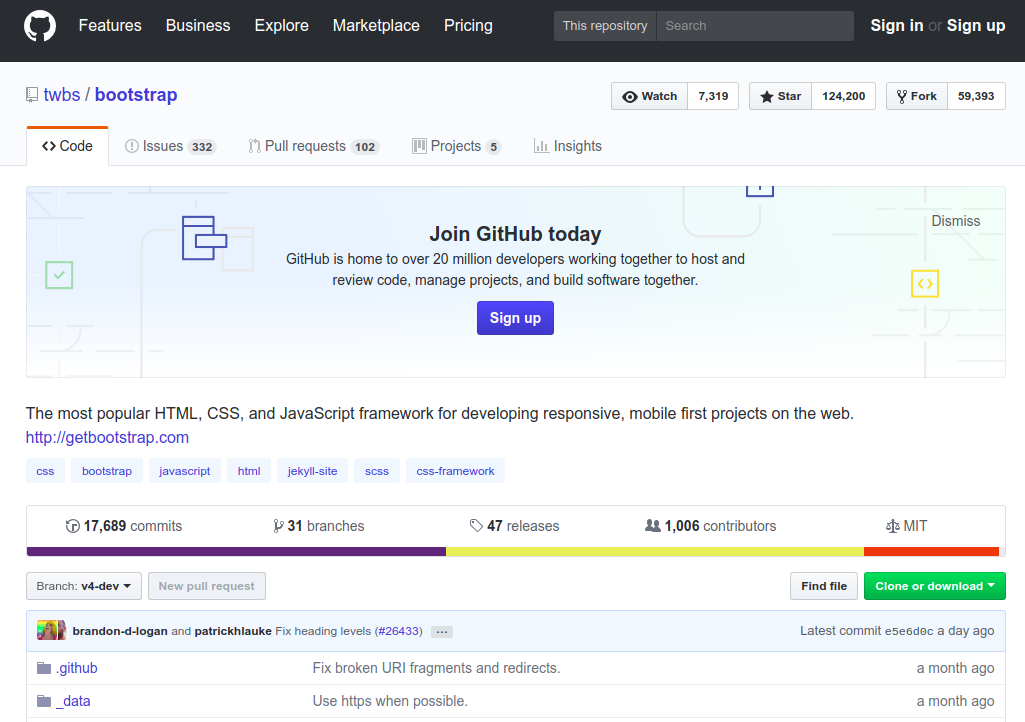
\includegraphics[height=0.7\paperheight]{print_github_1.png} \\
      \end{center}
 
\end{frame}
%--------------------------------------------------------------
\begin{frame}{Nome do projeto}
  \begin{center}
       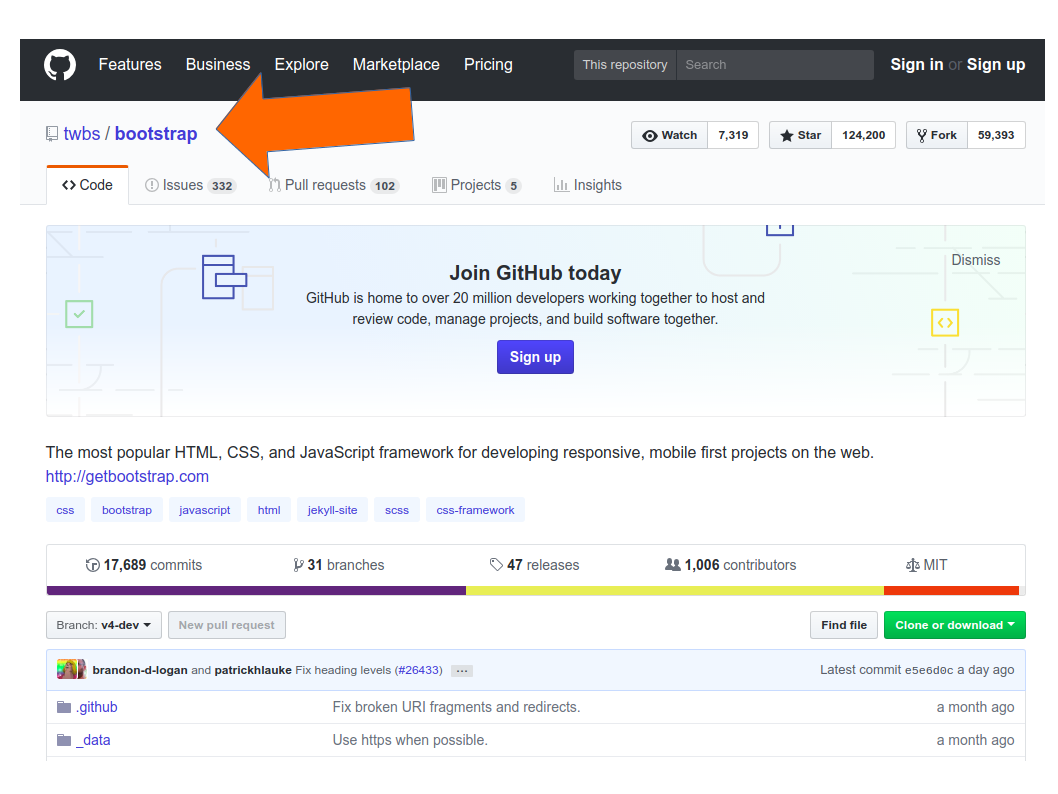
\includegraphics[height=0.7\paperheight]{nome_projeto.png} \\
      \end{center}
 
\end{frame}
%--------------------------------------------------------------
\begin{frame}{Visibilidade do projeto}
  \begin{center}
       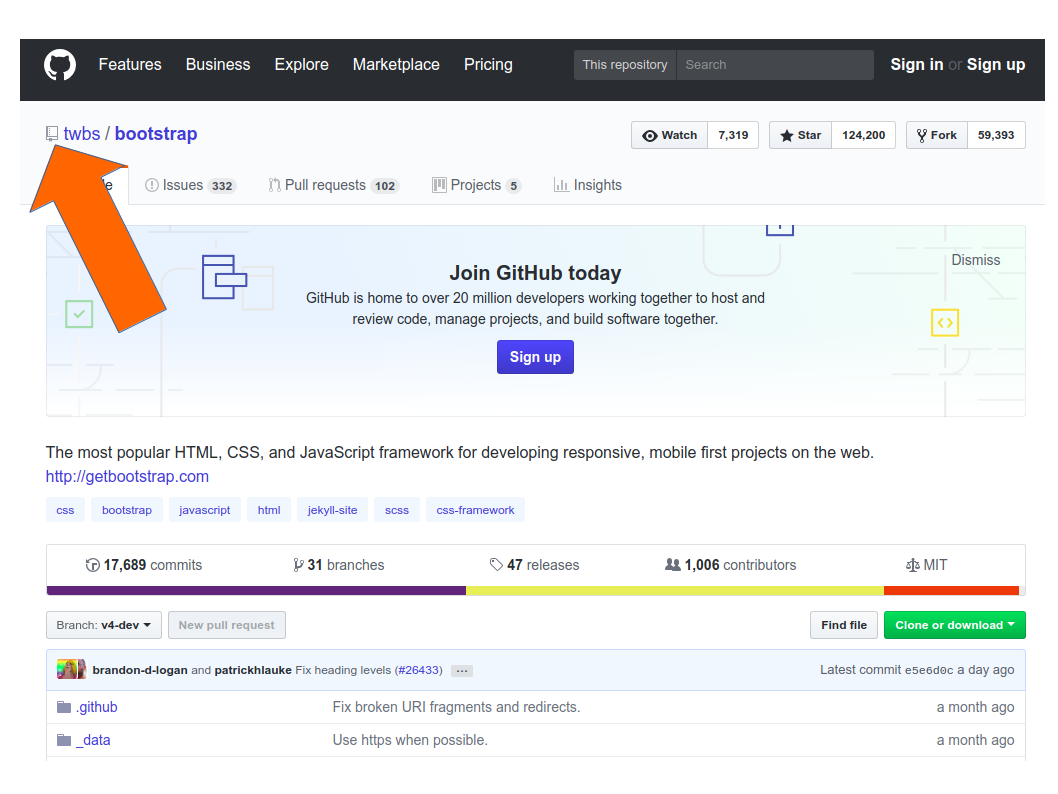
\includegraphics[height=0.7\paperheight]{visibilidade_projeto.png} \\
      \end{center}
 
\end{frame}
%--------------------------------------------------------------
\begin{frame}{Observadores do projeto}
  \begin{center}
       
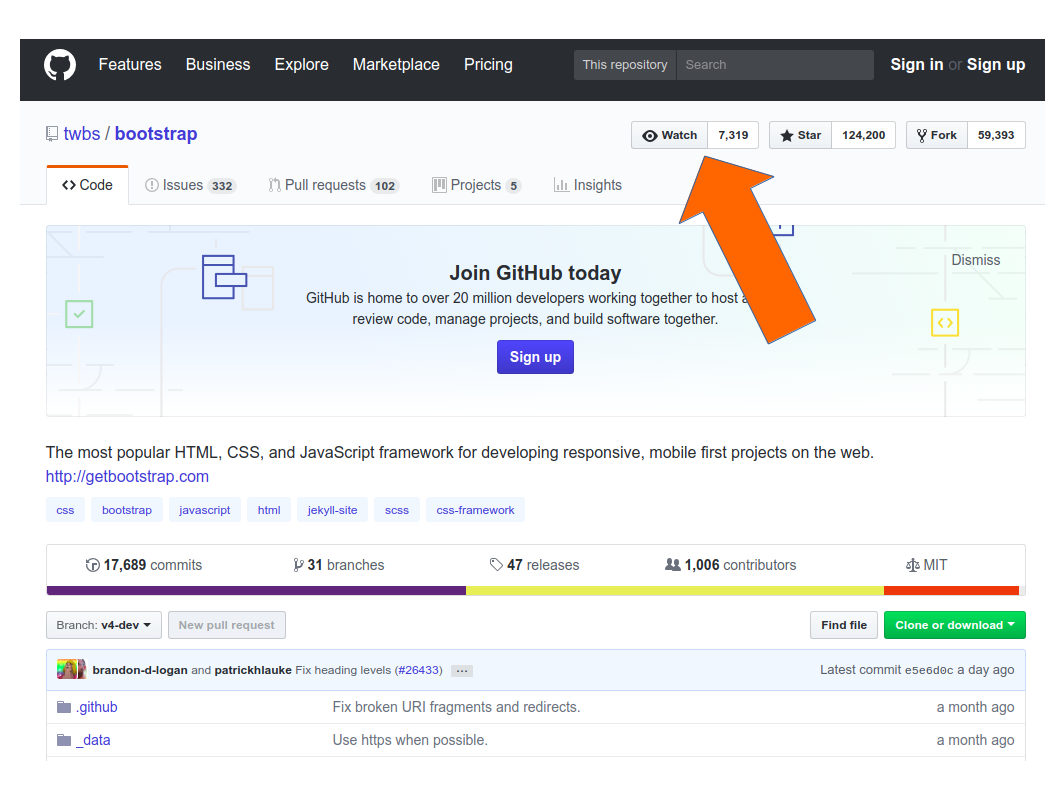
\includegraphics[height=0.7\paperheight]{views_projeto.png} \\
      \end{center}
 
\end{frame}
%--------------------------------------------------------------
\begin{frame}{Favorito}
  \begin{center}
       
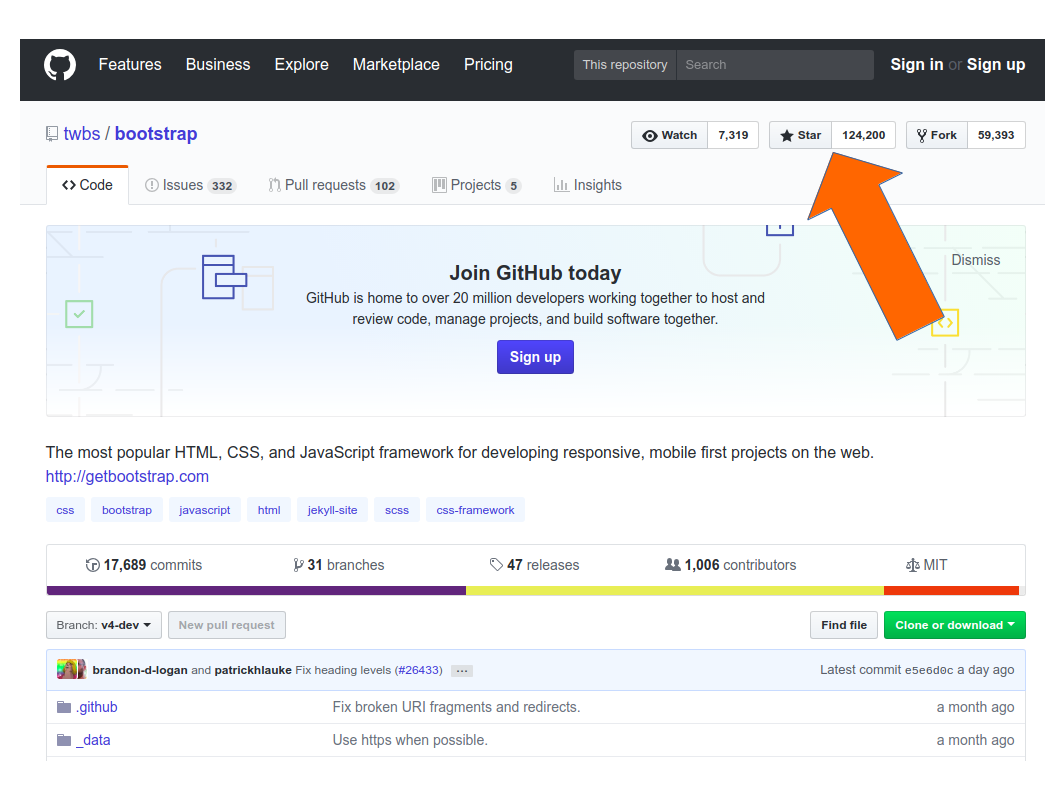
\includegraphics[height=0.7\paperheight]{favorito_projeto.png} \\
      \end{center}
 
\end{frame}
%--------------------------------------------------------------
\begin{frame}{Fork}
  \begin{center}
       
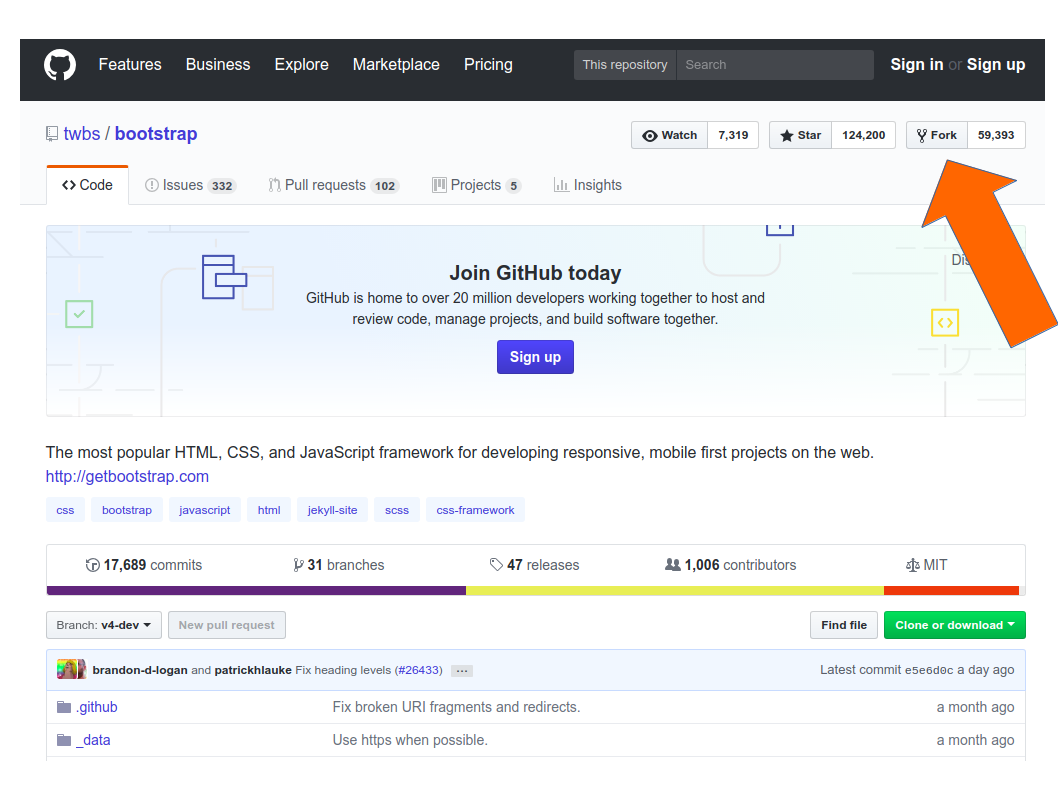
\includegraphics[height=0.7\paperheight]{fork_projeto.png} \\
      \end{center}
 
\end{frame}
%--------------------------------------------------------------
\begin{frame}{Commits}
  \begin{center}
       
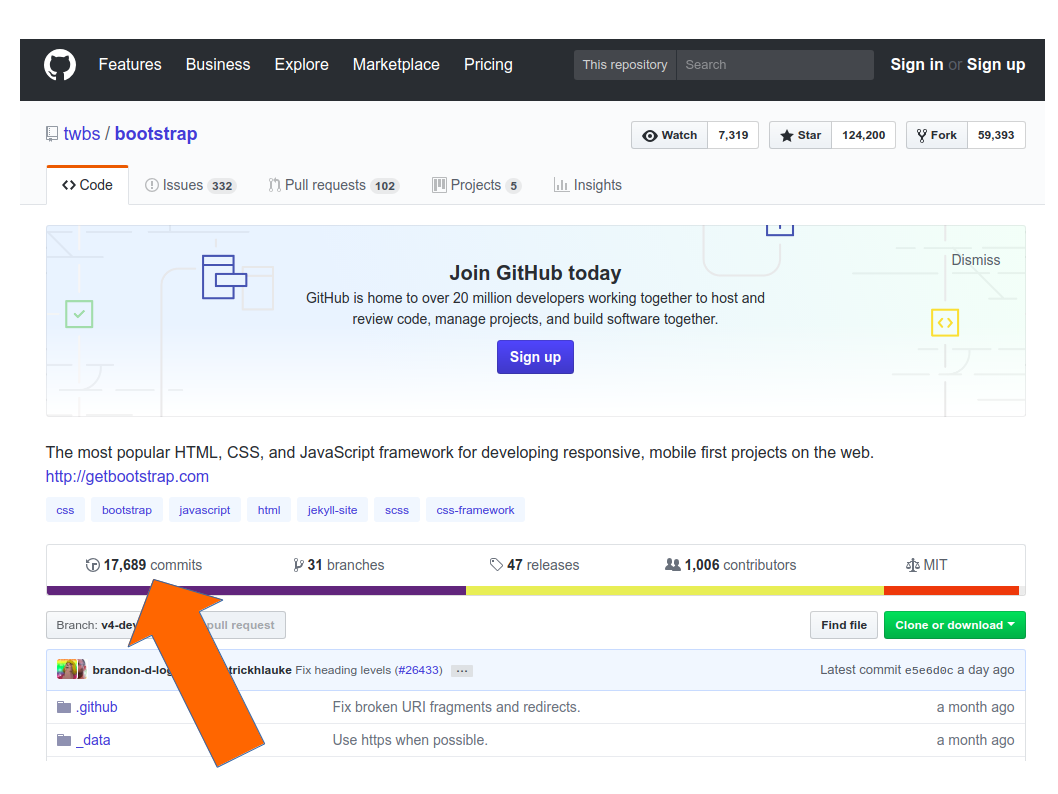
\includegraphics[height=0.7\paperheight]{commits_projeto.png} \\
      \end{center}
 
\end{frame}
%----------------------------------------------------------------------------
\section{Configurando VSCode com GitHub}
\begin{frame}{GitHub no VSCode}
\begin{itemize}
  \item Acesse o github e crie um repositório para colocar o projeto.
   \item Clone o projeto no VSCode.
   \item Faça o \textit{clone} do seu repositório GitHub, utilizando a opção "clonar repositório"na página inicial do VSCode.
   \end{itemize}
       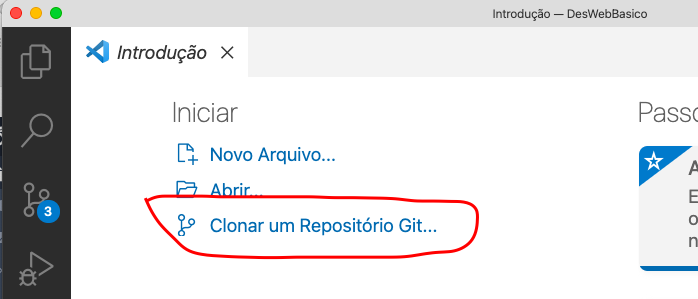
\includegraphics[height=0.4\paperheight]{fig/aula4/aula4_1.png} \\
       \tiny{VSCode Versionamento}.
     
\end{frame}
%----------------------------------------------------------------------------
\begin{frame}{Versionando com GitHub}
Crie a pasta docs e dentro dela o arquivo index.html no seu projeto;
\begin{itemize}
   \item Barra esquerda do projeto \textit{Controle do código fonte}
   \item Escolha a opção confirmar alterações
   \item Digite a mensagem do commit: "criando pasta docs";
   \item No repositório (navegador) acesse: Settings
   \item Escolha Pages;
   \item Cria a sua page, apontando para a pasta docs do repositório no GitHub;
\end{itemize}
\end{frame}


%-----------------------------------------------------------------
\section{GitHub}
\begin{frame}{GitHub}{Enviando modificações}
  \begin{itemize}
   \item Faça as edições necessárias na sua página HTML na pasta docs;
   \item O sistema de versionamento vai solicitar Commit
   \item Digite a mensagem do commit
   \item Escolha o Branch \textit{criado por você};
   \item Atualize a página do repositório no GitHub;
  \end{itemize}

\end{frame}
%-----------------------------------------------------------------
\section{Atividade de aula}
\begin{frame}{Atividade}{Envie seu repositório feito em aula}
  \begin{enumerate}
      \item Seguindo os passos da aula, livros indicados e, a leitura adicional recomendada: \textcolor{blue}{\href{https://docs.github.com/pt/pages/getting-started-with-github-pages/creating-a-github-pages-site}{Getting started with github pages}}, DESENVOLVA:
      \item Os passos realizados em aula;
      \item Envie no BlackBoard o link do repositório criado \textbf{em aula} e da GitHubPage;
  \end{enumerate}


\end{frame}
%-----------------------------------------------------------------------
\section{Leitura recomendada}
\begin{frame}{Leitura complementar}
 Para mais informações sobre Git e GitHub, leia:\\
  \vspace{0.6cm}
 \begin{columns}
   \begin{column}{0.4\textwidth}
%      \textbf{Capítulo 29}\\
 \cite{githubpages2022}\\
 E\\
 \cite{beer2015github}.
   \end{column}
   \begin{column}{0.4\textwidth}
    
\includegraphics[height=0.7\paperheight]{introgit.jpg} \\
   \end{column}

 \end{columns}
\end{frame}

%----------------------------------------------------------------------------
\section{Referências}

\begin{frame}{Referências}%[allowframebreaks]
\small
\begin{center}
\tiny
\bibliographystyle{apalike}
\bibliography{ref_aula}
\end{center}
\end{frame}

\end{document}

\end{document}